\documentclass[]{scrartcl}

\usepackage{\string~"/LaTeX/StylePackage"}

\title{Radiophysics Lab}
\author{}
\date{14.10.2024}


\begin{document}

\maketitle
\newpage
\tableofcontents
\newpage

In this Laboratory course we will learn how to work with basic radioactive sources, and how to measure and interpret data that comes about in the experiments. We will 


\section{X-Ray Tube}


\section{Preparatory measurements}

We will be making measurements of the X-Rays liberated electrons over time, to see how an increased or decreased time affects the amount of liberated electrons. We will be measuring over 15, 30 and 45 seconds. We will keep the Area that we measure over, and the Intensity with which the electrons arrive at our area of measurement equal. We then expect a relation of
\begin{equation}
	Q = \int \text dt\int \text dA I(r_0) = tAI(r_0),\;\;\; Q \propto t
\end{equation}
Measurement are made with 1.52mm aluminium filter. The tray is 30cm away from the source\\
The X-Ray tube shall be set to $120$ kV an $10$ mA. Measurements are in nC.

\begin{center}
	\begin{tabular}{||c||c|c|c||}
	\hline
		 & $15s$ & $30s$ & $45s$\\
	\hline
		Measurements & 8.25 & 18.27 & 28.06 \\
		     	& 8.3 & 17.89 & 27.72 \\
			& 8.44 & 18.14 & 27.97\\
			& 8.31 & 18.04 & 27.51\\
			& 8.52 & 18.68 & 27.55\\
	\hline
		Average & 8.364 & 18.204 & 27.762\\
	\hline
		Average of Squared & 69.966 & 331.458 & 770.778\\
	\hline
		Standard Deviation & 0.097 & 0.269 & 0.222\\
	\hline
	\end{tabular}
\end{center}
with the average and standard deviation:
\begin{gather}
	\langle\mu\rangle = \frac{\sum_i^n x_i}{n},\;\;\;\;
	\sigma = \sqrt{\langle\mu^2\rangle - \langle\mu\rangle^2}
\end{gather}
In relation to the Average, the Standard deviation goes down with increasing time, signifying a more accurate measurement. We also notice that there is a linear increase with time. This linear increase signifies the charge that is picked up. We can read off a slope of 0.64$nC/s$.

\begin{centering}
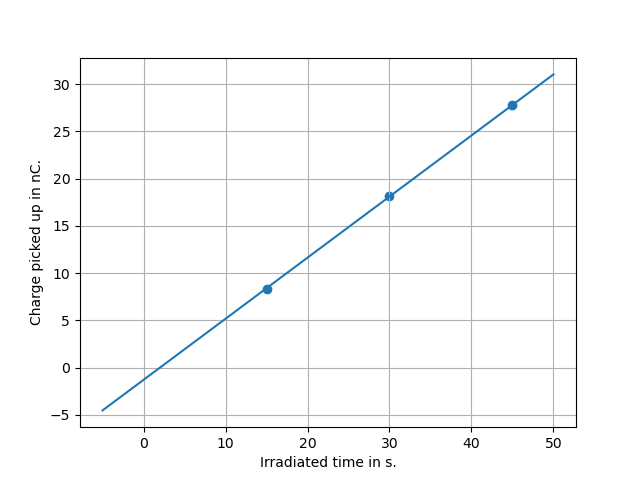
\includegraphics[width=15cm]{PrepMeasure}
\end{centering}
Such that we know that the Radiator sends off $0.64nC$ of charge every second.
\section{Inverse square law}


Measuring the charge that is registered by a surface at different distances away from the source we can gather information about the relationship between Intensity of a field and distance away from the source. We assume that our findings will line up with the Inverse square law, so that $I(r) = I_0\frac{1}{r^2}$, where $r$ is the distance away from the center. This comes from the fact that we are measuring an Electromagnetic Wave, which is governed by $E = \frac{1}{4\pi\epsilon}\frac{Q}{r^2}$.\\

We will measure for 30s with the previous filter of 1.52mm, we will start at 30cm and end at 60cm in 5cm intervals. We use the previous measurement for 30cm.

\begin{center}
	\begin{tabular}{||c|c||}
		\hline
		Distance [cm] & Charge [-nC] \\
		30 & 18.00\\
		35 & 13.48\\
		40 & 10.36\\
		45 & 8.44\\
		50 & 6.91\\
		55 & 5.52\\
		60 & 4.74\\
		\hline
	\end{tabular}
\end{center}

Plotting the Charge against the inverse square of the distance should give a linear plot.

\section{Exponential photon attenuation}
The Photon attenuation law is a law that concerns the resulting intensity when photons travel through a Medium. Mathematically we state this as
\begin{equation}
	N_x = N_0 \exp(-\mu x)
\end{equation}
where $N_x$ is the amount of photons after interacting with the medium, and $N_0$ is the incoming amount of photons. $\mu$ is the linear attenuation coefficient, and represents how much Intensity is lost through the medium per distance, it has units $1/m$. $x$ is the distance that the photons travel through.

We can reduce this equation to a linear equation in x, so that we can determine the coefficient $\mu$ by using the relation
\begin{equation}
	\ln(N_x/N_0) = -\mu\cdot x
\end{equation}
So, we will use the logarithm of Intensity that is left and graph it against the length of the medium through which it travelled. The resulting linear fit will give us a coefficient $y = mx$ with $m=\mu$. We will pick $N_0$ such that the first measurement of $N_x = N_0$. This will result in a linear fit where we can ignore the coefficient $b$ in
\begin{equation}
	\ln(N_x/N_0) = -\mu\cdot x + b
\end{equation}

We will put the measuring device at 30cm
\begin{center}
\begin{tabular}{|c|c|}
\hline
	Material Width [mm] & Charge [-nC]\\
	\hline
1.52 &  18.00\\
2.02 &  16.14\\
2.52 &  14.54\\
3.02 &  13.11\\
4.02 &  11.05\\
\hline
\end{tabular}
\end{center}


\section{Ionizations and radiation dose}

\begin{figure}
	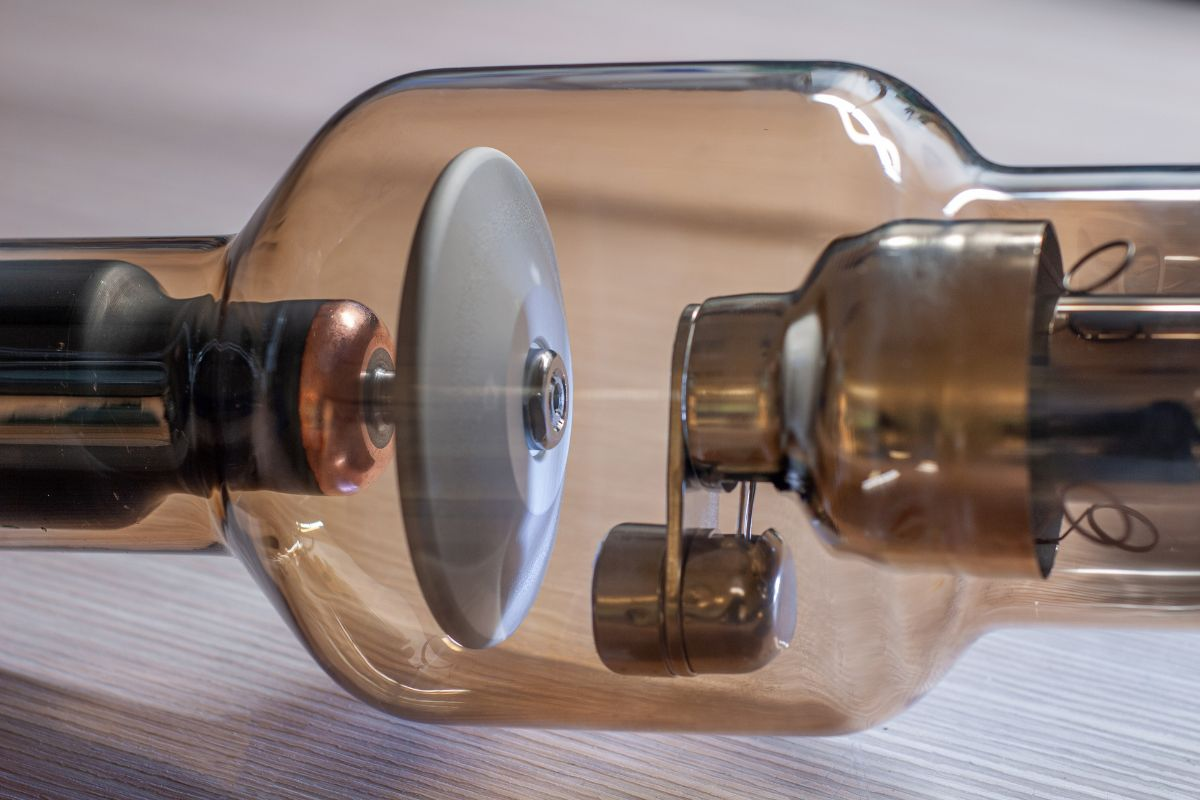
\includegraphics[width=15cm]{XRayTube}
\end{figure}


\end{document}

